\documentclass{article}

\usepackage{PRIMEarxiv}

\usepackage[utf8]{inputenc} % allow utf-8 input
\usepackage[T1]{fontenc}    % use 8-bit T1 fonts
\usepackage{hyperref}       % hyperlinks
\usepackage{url}            % simple URL typesetting
\usepackage{booktabs}       % professional-quality tables
\usepackage{amsfonts}       % blackboard math symbols
\usepackage{amsmath}
\usepackage{amssymb}
\usepackage{nicefrac}       % compact symbols for 1/2, etc.
\usepackage{microtype}      % microtypography
\usepackage{fancyhdr}       % header
\usepackage{graphicx}       % graphics
\usepackage{float}          % [H] placement for the contribution table
\usepackage{capt-of}        % captions for side-by-side figure and table
\graphicspath{{media/}}     % organize your images and other figures under media/ folder

% Shorthand
\newcommand{\R}{\mathbb{R}}
\newcommand{\E}{\mathbb{E}}

%Header
\pagestyle{fancy}
\thispagestyle{empty}
\rhead{ \textit{ }}

% Update your Headers here
\fancyhead[LO]{Multi-Agent RL in a Fishery Markov Game}

%% Title
\title{Multi-Agent Reinforcement Learning in a Fishery Markov Game with Unknown Regrowth}

\author{
  Panchal Heet Chirag, Param Tanna, Mehul Prakash Parakh, Pawar Sai Tejeshwar \\
  CS-329 Multi-Agent Systems \\
  IIT Gandhinagar \\
  \texttt{\{heet.panchal, param.tanna, mehul.parakh, pawar.sai\}@iitgn.ac.in} \\
  Code, data and results: \url{https://github.com/ParamTanna/Fishery-Marl} \\
}

\begin{document}
\maketitle

\begin{abstract}
Two fishing fleets share one lake. Each season every fleet decides how much to catch, and the fish that are left regrow before the next season, at a rate the fleets do not know, so they must learn how to harvest while the other fleet learns as well. We model this as a Markov game with an unknown transition kernel, compute the social planner's solution and the Markov perfect equilibria exactly, certifying every equilibrium by an exact best response, and measure how far learning fleets end up from both, what happens to the fish stock, and what learning costs. The tragedy is real but moderate: the Price of Anarchy is 1.16 at $r=0.5$ and 1.04 at $r=0.8$. Independent Q-learners end far below any equilibrium and collapse the stock in almost every run. A Bayesian model-based fleet reaches the equilibrium it plays, and a fleet that best-responds to a learned model of the other settles near the planner without collapse and gains $+1436.5\pm331.3$ against an over-harvester. A reserve cap removes collapse but costs the equilibrium 142--563 and the planner nothing. Cooperation at the planner's catch is subgame perfect under a grim trigger for $\gamma\ge\gamma^*\approx0.68$--$0.77$, yet memory-one learners do not discover it.
\end{abstract}

\keywords{Multi-agent reinforcement learning \and Markov games \and Tragedy of the commons \and Learning under uncertainty}

%------------------------------------------------------------
\section{Introduction}
%------------------------------------------------------------
Shared resources such as fisheries, groundwater and grazing land are often overused, even when every user would be better off with restraint. Hardin \cite{hardin1968} called this the tragedy of the commons: each user gets the full benefit of taking more but bears only a share of the damage, so self-interested users end up worse off than a planner could make them. Ostrom \cite{ostrom1990} showed that real communities sometimes avoid this outcome, which raises the question of when restraint can emerge among the users themselves.

Fish regrow, so what is caught today changes what is available tomorrow. The natural model is therefore a Markov game \cite{littman1994}, the multi-agent version of a Markov decision process (also called a stochastic game \cite{shapley1953}). The classic ``Great Fish War'' \cite{levhari1980} studies such a game, but it assumes that everyone knows the growth law and can compute equilibrium strategies. Real fleets observe only the stock and the catches, and they learn by experience.

This makes the problem one of multi-agent reinforcement learning (MARL) \cite{zhang2021}. From the point of view of one agent the others are part of the environment and keep changing as they learn, so the environment is not stationary and the convergence guarantee of Q-learning \cite{watkins1992} no longer applies to independent learners \cite{tan1993}. Common-pool resources have been studied with deep agents in rich environments \cite{leibo2017,perolat2017}; we instead use a small model whose benchmarks can be computed exactly, so that we can tell how good the learned behaviour really is.

\medskip
\noindent\textbf{Research question.} \textit{When several reinforcement learning agents share a renewable resource whose regrowth rate they do not know, how close do their learned policies get to the socially best harvest, what happens to the fish stock, and what does the learning cost?}
\medskip

We break this into four sub-questions.
\begin{enumerate}
\item \textbf{Where do learners settle?} Do independent learners approach the equilibrium, the planner's solution, or something else, and how does this depend on $r$, the number of fleets and $\gamma$?
\item \textbf{Does the learning method matter?} Do centralised critics or explicit models help compared with independent learners, in samples needed and in final return?
\item \textbf{What does not knowing $r$ do?} Do fleets over- or under-harvest compared with fleets that know $r$, and how large is the risk of collapse, including during exploration?
\item \textbf{Can cooperation emerge?} If policies can react to the previous stock and catches (memory-one policies $\pi_i(a^i\mid s_t,s_{t-1},\hat a_{t-1})$), do learners find threats and punishments, such as a grim trigger, that sustain restraint?
\end{enumerate}
Sections~\ref{sec:prelim} and~\ref{sec:formulation} define the game, Section~\ref{sec:solutions} recalls the plan, Sections~\ref{sec:method} and~\ref{sec:results} give the methods and results, and Section~\ref{sec:contrib} the division of work.

%------------------------------------------------------------
\section{Preliminaries}
\label{sec:prelim}
%------------------------------------------------------------
\paragraph{Markov game.} A Markov game is a tuple $\langle \mathcal N, \mathcal S, \mathcal A, P, R, \gamma\rangle$. In each round the agents $\mathcal N$ see the state $s\in\mathcal S$, each agent $i$ picks an action $a^i$, giving the joint action $a=(a^1,\dots,a^{|\mathcal N|})$, and receives a reward $R_i(s,a)$. The next state is drawn from $P(s'\mid s,a)$ and future rewards are discounted by $\gamma\in(0,1)$. A policy $\pi_i(a^i\mid s)$ says how agent $i$ acts in each state, and $\pi=(\pi_1,\dots,\pi_{|\mathcal N|})$ is a joint policy.

\paragraph{Values and solution concepts.} Let $\rho_0$ be the initial-stock distribution. For $\pi=(\pi_i,\pi_{-i})$,
\begin{equation}
V_i^{\pi}(s)=\mathbb{E}_{\pi}\Big[\sum_{t\ge0}\gamma^{t}R_i(s_t,a_t)\,\Big|\,s_0=s\Big],\qquad
J_i(\pi)=\mathbb{E}_{s\sim\rho_0}\big[V_i^{\pi}(s)\big].
\end{equation}
$\pi^{*}$ is a \emph{Nash equilibrium} if $J_i(\pi_i,\pi^{*}_{-i})\le J_i(\pi^{*})$ for all $i$ and $\pi_i$, and a \emph{Markov perfect equilibrium} (MPE)~\cite{maskin2001} if each $\pi^{*}_i$ depends only on the current state and
\begin{equation}
V_i^{(\pi_i,\pi^{*}_{-i})}(s)\le V_i^{\pi^{*}}(s)\qquad\forall\, i,\ \forall\,\pi_i,\ \forall\, s\in\mathcal S,
\end{equation}
i.e.\ no agent gains by deviating from \emph{any} state. A planner policy is $\pi^{\mathrm{plan}}\in\arg\max_{\pi}\sum_{i}J_i(\pi)$; the gap between $\sum_i J_i(\pi^{\mathrm{plan}})$ and $\sum_i J_i(\pi^{*})$ is the loss caused by selfishness.

\paragraph{Learning with an unknown kernel.} If $P$ depends on an unknown parameter $r$, an agent can keep a belief $b_t(r)$ and update it after each transition by Bayes' rule,
\begin{equation}
b_{t+1}(r)\;\propto\;P_r(s_{t+1}\mid s_t,a_t)\,b_t(r),
\end{equation}
and a good policy conditions on both the state and the belief, $\pi(a\mid s,b)$.

\paragraph{Memory and punishment.} A policy that sees only the current state cannot react to what the others did. Memory-one policies $\pi_i(a^i\mid s_t,s_{t-1},\hat a_{t-1})$ also see the previous stock and joint executed catch. A classic example is the grim trigger: take the planner's share as long as everyone has done so, and switch to the selfish equilibrium forever after the first deviation. Whether such a threat sustains restraint depends on how patient the agents are, that is, on $\gamma$.

\paragraph{Learning by interaction.} \emph{Independent Q-learning} treats the other agents as part of the environment \cite{tan1993,watkins1992}; \emph{actor-critic} methods follow the gradient of a parametrised policy \cite{sutton2018}; \emph{centralised training with decentralised execution} lets the critic see all agents' actions during training \cite{lowe2017}; \emph{model-based} learners estimate the unknown parameter and plan in the estimated game. Nash Q-learning~\cite{hu2003} is a model-free relative that plays a Nash equilibrium of learned joint-action values.

%------------------------------------------------------------
\section{Problem Formulation}
\label{sec:formulation}
%------------------------------------------------------------
\paragraph{Agents, state and actions.} $\mathcal N=\{1,2\}$ are the fishing fleets and $\mathcal S=[0,K]$ is the fish stock at the start of a season. Each fleet requests a catch $a^i\in[0,K]$; if the requests exceed the stock they are scaled down proportionally,
\begin{equation}
\hat a^i(s,a)=a^i\cdot\min\Big\{1,\ \frac{s}{\sum_j a^j}\Big\},
\end{equation}
with $\hat a^i=0$ if nobody requests anything, so $\sum_i\hat a^i\le s$. When the lake is scarce a larger request earns a larger share, which creates a race to fish.

\paragraph{Reward.} $R_i(s,a)=p\,\hat a^i-\frac{c}{2}\,(\hat a^i)^2$ with $p,c>0$: revenue minus a convex effort cost, which keeps the best catch from being ``take everything''.

\paragraph{Transition (unknown to the agents).} The fish left after fishing, $x=s-\sum_i \hat a^i$, regrow logistically and are hit by lognormal noise with mean one:
\begin{equation}
s'=\min\Big\{K,\ \omega\cdot g_r(x)\Big\},\qquad g_r(x)=x+r\,x\Big(1-\frac{x}{K}\Big),\qquad \omega=\exp\big(\sigma\xi-\tfrac{\sigma^2}{2}\big),\ \ \xi\sim\mathcal N(0,1).
\end{equation}

\paragraph{Known and unknown.} Known: $K,p,c,\sigma,\gamma,\rho_0$. Observed each season: $s_t$, all executed catches and the own reward. Unknown: the regrowth rate $r$ and the other fleet's policy. Since one noiseless transition reveals $r$, all unknown-$r$ experiments use $\sigma>0$. Only the model-based learner is given the form of $P$; it updates a public belief over $r$ from each pair $(x_t,s_{t+1})$ with the lognormal density for $s_{t+1}<K$ and the censored mass $\ell_r=1-\Phi\big((\log(K/g_r(x_t))+\sigma^2/2)/\sigma\big)$ at $s_{t+1}=K$.

\paragraph{Benchmarks (known $r$).} $\pi^{\mathrm{plan}}\in\arg\max_{\pi}\sum_i J_i(\pi)$ and $\pi^{\mathrm{eq}}$, a symmetric Markov perfect equilibrium; when several exist we report all of them. A fleet does not count the damage its catch does to the other through next season's stock, so we expect equilibrium catches to be at least the planner's and the long-run stock to be lower; this is not guaranteed in general~\cite{dutta1993}.

\paragraph{Learning problem (unknown $r$).} Fleet $i$ maps its history to a policy $\pi^t_i$. With $\pi^{\mathrm{ref}}\in\{\pi^{\mathrm{eq}},\pi^{\mathrm{plan}}\}$ and $t$ counting seasons over training, we measure
\begin{align}
G(\pi^t)&=1-\frac{\sum_i J_i(\pi^t)}{\sum_i J_i(\pi^{\mathrm{plan}})} &&\text{(efficiency gap)}\\
E(\pi^t)&=\max_{i}\Big[\max_{\pi_i}J_i(\pi_i,\pi^t_{-i})-J_i(\pi^t)\Big] &&\text{(distance to equilibrium)}\\
C_T(\pi^t)&=\Pr\nolimits_{\pi^t}\Big(\min_{0\le k\le T}s_k<\delta K\Big) &&\text{(collapse probability)}\\
L_\tau&=\sum_{t=0}^{\tau}\Big[\sum_i J_i(\pi^{\mathrm{ref}})-\sum_i J_i(\pi^t)\Big] &&\text{(cost of learning)}
\end{align}
and the long-run stock. The \emph{safe version} solves the same problems subject to $C_T(\pi)\le\kappa$ for a finite horizon $T$; over an infinite horizon a dip below $\delta K$ has probability one under every policy when $\sigma>0$.

\paragraph{Remark.} A fleet's one-season optimum is $\hat a^i=p/c$ and the largest sustainable total catch is $rK/4$ for $r\le2$. If $|\mathcal N|\,p/c\le rK/4$ selfishness costs nothing, so we choose $|\mathcal N|\,p/c>rK/4$: $r$ decides whether a tragedy exists at all.

%------------------------------------------------------------
\section{Proposed Solutions}
\label{sec:solutions}
%------------------------------------------------------------
At the project review we planned the following. (i) A fishery environment with the proportional rationing rule and exact benchmarks for known $r$: the planner by dynamic programming and the equilibrium by solving a small game between the fleets in every state (pure profiles first, Lemke--Howson otherwise), validated on the Levhari--Mirman specification~\cite{levhari1980} (reward $\log\hat a^i$, growth $s'=x^{\alpha}$, $\sigma=0$), whose planner harvests $(1-\alpha\gamma)s$ and whose symmetric equilibrium has each of $n$ fleets harvest $\frac{1-\alpha\gamma}{n-(n-1)\alpha\gamma}\,s$, to within 1\%. (ii) Learners: independent Q-learning, independent actor-critic, a centralised critic, a model-based learner that keeps a belief over $r$ and plays the equilibrium of the estimated game, and a team-reward baseline. (iii) Experiments with 50-season episodes from $s_0=K$ (a truncation: learners bootstrap from the last stock), varying $r$, the number of fleets, $\gamma$, $\sigma$, the learning method, exploration and the amount of data, over at least 10 seeds with 95\% confidence intervals, and tracking collapse during training as well as after it. (iv) A memory-one test: force a one-season over-harvest and check whether the other fleet punishes and then returns to restraint. The neural learners, three fleets and the memory experiments were extensions, to be dropped first if time ran short. The project succeeds if every research question is answered with these measurements, whether or not the learners reach the benchmarks.

%------------------------------------------------------------
\section{Methodology}
\label{sec:method}
%------------------------------------------------------------
We use $K=100$, $p=10$, $c=2/3$ ($p/c=15$), $\gamma=0.99$, $\sigma=0.1$, $\delta=0.2$, $\kappa=0.05$, $T=50$, $s_0=K$,
and $r\in\{0.5,0.6,0.7,0.8\}$, with $r=1.5$ as a no-tragedy control ($|\mathcal N|\,p/c=30>rK/4$ for every $r\le0.8$).
\textbf{Changes from the plan of Section~\ref{sec:solutions}:} the equilibrium is computed as a stationary fixed point
with an exact certificate rather than by finite-horizon backward induction; all stage equilibria are reported (review
feedback 2); an opponent-aware learner and a cross-play tournament were added (review feedback 1); the centralised critic
is tabular; the exploration schedule was tuned on seeds 0--2 rather than swept; the neural actor-critic and the
three-fleet case, both planned as optional extensions, were not run. Experiments are numbered E0--E12 as in the
repository README.

\subsection{Exact benchmarks}
Stock and catch are discretised on uniform grids over $[0,K]$ with 101 and 51 points ($\Delta s=1$, $\Delta a=2$).
$\E[V(s')]$ uses 21-node Gauss--Hermite quadrature over $\xi$, with the probability mass above $K$ placed on $s'=K$
analytically, and linear interpolation between stock nodes. The \textbf{planner} is a single-agent MDP over joint catches
($51^2$ actions per state), solved by Howard policy iteration~\cite{howard1960} with exact policy evaluation.

\textbf{Equilibria.} Given continuation values $V_i$, the stage game at stock $s$ is the bimatrix
$U_i(s,a^1,a^2)=R_i(s,a)+\gamma\,\E[V_i(s')]$. Algorithm~1 alternates between choosing, in every state, one stage
equilibrium by a selection rule and evaluating the resulting stationary profile exactly, which searches directly for a
stationary MPE of the infinite-horizon game. Seven rules are used: maximum total payoff (the rule planned in
Section~\ref{sec:formulation}), minimum total payoff, payoff dominance, risk dominance~\cite{harsanyi1988}, maximum
catch, continuity with the previous iterate, and seeded random choice. Lemke--Howson~\cite{lemke1964} is used only on
small grids (the Levhari--Mirman test); on the fishery grid, enumeration is exact and cheaper. Every returned profile
$\pi$ is then \textbf{certified} against the definition of an MPE: for each fleet the exact best response to $\pi_{-i}$
is computed by Howard policy iteration, giving
\begin{equation}\label{eq:cert}
E(s)=\max_{\pi_i}V_i^{(\pi_i,\pi_{-i})}(s)-V_i^{\pi}(s)\quad\text{at every stock } s,
\end{equation}
and $\pi$ is accepted when $E(s)\le1$ everywhere or $E\le10^{-3}$ of the fleet's value. With $\Pi^*$ the set of
certified equilibria, the Price of Anarchy and the Price of Stability~\cite{koutsoupias1999,anshelevich2004} are
\begin{equation}\label{eq:poa}
\mathrm{PoA}=\frac{\sum_i J_i(\pi^{\mathrm{plan}})}{\min_{\pi^*\in\Pi^*}\sum_i J_i(\pi^*)},\qquad
\mathrm{PoS}=\frac{\sum_i J_i(\pi^{\mathrm{plan}})}{\max_{\pi^*\in\Pi^*}\sum_i J_i(\pi^*)}.
\end{equation}

\begin{table}[H]
\centering
\small
\begin{tabular}{p{15.5cm}}
\toprule
\textbf{Algorithm 1.} Symmetric MPE by selection and evaluation (selection rule $\rho$) \\
\midrule
1: $V\leftarrow 0$, $\pi\leftarrow$ zero catch \\
2: \textbf{repeat} for each stock $s$: build $U(s,\cdot,\cdot)$ from $V$; $\mathcal E(s)\leftarrow$ pure NE $\cup$ symmetric 2-support mixed NE; $\pi(s)\leftarrow\rho(\mathcal E(s),\pi)$; \\
\quad\ \ then $V\leftarrow$ exact value of $(\pi,\pi)$ \\
3: \textbf{until} $\pi$ is unchanged, or exploitability has not fallen for 8 rounds (then keep the least exploitable $\pi$) \\
4: certify $\pi$ with Eq.~\eqref{eq:cert} at every stock \\
\bottomrule
\end{tabular}
\end{table}

\subsection{Learners}
All learners act on the same grids and train in 50-season episodes from $s_0=K$, bootstrapping from the value of the
last stock (Section~\ref{sec:solutions}).
\textbf{IQL}: tabular Q-learning over (stock, own catch), $\varepsilon$-greedy with $\varepsilon$ decaying from 0.5 to
0.02, 5000 episodes.
\textbf{MB-EQ} (model-based, plays the equilibrium): the Bayesian belief of Section~\ref{sec:formulation} on 191 values of
$r\in[0.1,2]$; five exploratory warm-up seasons per episode, then the precomputed equilibrium policy at the posterior mean,
interpolated between the solved values of $r$ and re-planned every 5 seasons; 500 episodes.
\textbf{MB-OA} (model-based, opponent-aware; review feedback 1): the same belief plus a kernel-smoothed model of the other
fleet's \emph{request} as a function of stock (bandwidth 5), recovered from executed catches by inverting the rationing
rule; it plays the exact best response to that model in the estimated game (Howard policy iteration, re-planned every 5
seasons); 200 episodes.
\textbf{Team baselines}: Team-IQL is IQL on the total reward; Team-Planner plays the planner policy at the posterior mean
(an oracle reference).
\textbf{Joint-action critic (CTDE)}: tabular $Q(s,a^1,a^2)$ learned from both fleets' catches during training; each fleet
executes its own action against a model of the other~\cite{claus1998}.
\textbf{Memory-one}: tabular Q-learning whose state adds a regime bit that turns on when the other fleet's last catch
exceeded $\mathrm{clip}(0.1\,s,2,10)$.

\subsection{Safe version, cooperation threshold and evaluation}
\textbf{Safe version.} Each fleet's catch is capped at $a^i\le\max(0,0.5(s-S_{\mathrm{res}}))$, so the joint catch never
pushes the stock below $S_{\mathrm{res}}$; $S_{\mathrm{res}}=25$ is the smallest value meeting $C_{50}\le\kappa$ on
tuning seeds $\{0,1,2\}$. Equilibria of the capped game are solved and certified with best responses restricted to legal
catches.

\textbf{Cooperation threshold.} Let $a^{\mathrm{coop}}(s)$ be the symmetric planner's catch (both fleets take the same
catch, chosen to maximise the total return) and let the punishment be a certified MPE $\pi^*$. Because the punishment
phase is itself an MPE, the one-shot deviation principle~\cite{fudenberg1986,abreu1988} says the grim trigger of
Section~\ref{sec:prelim} is a subgame-perfect equilibrium if and only if, at every stock and for each fleet,
\begin{equation}\label{eq:grim}
V_i^{\mathrm{coop}}(s)\ \ge\ \max_{a^i}\Big[R_i\big(s,a^i,a^{\mathrm{coop}}_{-i}(s)\big)+\gamma\,\E\big[V_i^{\pi^*}(s')\big]\Big].
\end{equation}
We evaluate Eq.~\eqref{eq:grim} exactly on a grid of $\gamma$, re-solving $\pi^*$ at each $\gamma$, and refine the
smallest $\gamma$ at which it holds, $\gamma^*(r)$, by bisection.

\textbf{Evaluation.} Hyperparameters were tuned on seeds $\{0,1,2\}$ and frozen; every reported number uses seeds 10--29
(20 seeds) with 95\% $t$-intervals. $J$ is computed by exact policy evaluation and by 500 Monte Carlo rollouts with
common random numbers, $E$ by exact best response, and $C_{50}$ by Monte Carlo. The cost of learning is reported per
episode, $\bar L_\tau=L_\tau/\tau$, against the planner's 50-season return. Cross-play differences are paired (same seed,
same noise) and tested per $r$ with Holm's correction~\cite{holm1979}.


%------------------------------------------------------------
\section{Results}
\label{sec:results}
%------------------------------------------------------------
% Every table below is generated by analysis/make_paper_assets.py from results/raw and the exact-analysis files.
\subsection{Exact benchmarks and equilibrium multiplicity}
\textbf{Validation.} On the Levhari--Mirman specification the solver reproduces the closed-form planner and equilibrium
policies within 0.95\% (target 1\%; $81\times401$ grid). Our planner, best responses and Bayesian filter also agree with
a separate re-implementation written from the model equations to $10^{-6}$, $10^{-10}$ and $10^{-15}$ respectively.

\textbf{Benchmarks.} Table~\ref{tab:bench} and Figure~\ref{fig:bench}(a) give the exact benchmarks. Stage games have
several equilibria in 16--71\% of stocks, so the selection rule matters. Three rules (minimum total, maximum catch,
continuity) return profiles that pass the certificate at every stock; they form the \emph{certified MPE band}. The tragedy
is real but moderate: $\mathrm{PoA}=1.160$ at $r=0.5$ and $1.041$ at $r=0.8$, and the band is narrow (PoA and PoS differ
by at most 0.011). The rule that keeps the highest-total stage equilibrium in every state, which we planned to use in the
project review, does \emph{not} give an equilibrium of the dynamic game at $r\le0.7$: a fleet gains 1030 by deviating from it
at full stock. Each state's choice is locally good but ignores how the other fleet's future play changes, so we
report it only as a ``stage-greedy'' reference. At $r=1.5$ there is no tragedy: all rules give the planner's value
($J=14933.3$). As anticipated in Section~\ref{sec:formulation}, certified equilibrium catches are at least the planner's
at every stock (one exception, by 0.3 units at one stock at $r=0.6$), so the long-run stock is lower: 41--55 under the
certified equilibria against 61--70 under the planner (Figure~\ref{fig:bench}(b,c): the planner rests the stock at low
levels and harvests above it, while selfish fleets keep fishing lower down). The planner's own policy is very exploitable ($E=446$--$1165$):
cooperation is efficient but not self-enforcing, which motivates Section~\ref{sec:coop}.

\begin{table}[h]
\centering
\caption{Exact benchmarks (known $r$). Band over the certified symmetric MPEs; PoA and PoS from Eq.~\eqref{eq:poa}.}
\label{tab:bench}
\small
\begin{tabular}{cccccccc}
\toprule
 & Planner & Certified MPE band & & & Planner & \multicolumn{2}{c}{Stage-greedy (max-total)} \\
$r$ & $J^{\text{plan}}$ & $[\min,\max]\,J^{*}$ & PoA & PoS & exploitability $E$ & $J$ & $E$ (not an MPE) \\
\midrule
0.5 & 9{,}802.5 & 8{,}452.7--8{,}532.6 & 1.160 & 1.149 & 1{,}164.9 & 7{,}607.0 & 1{,}030.2 \\
0.6 & 11{,}103.6 & 9{,}743.9--9{,}821.2 & 1.140 & 1.131 & 912.1 & 8{,}275.8 & 271.6 \\
0.7 & 12{,}204.1 & 11{,}437.1--11{,}474.4 & 1.067 & 1.064 & 658.9 & 10{,}615.1 & 95.2 \\
0.8 & 13{,}106.6 & 12{,}584.6--12{,}614.7 & 1.041 & 1.039 & 445.9 & 12{,}369.9 & 10.8 \\
\bottomrule
\end{tabular}

\end{table}

\begin{figure}[h]
\centering
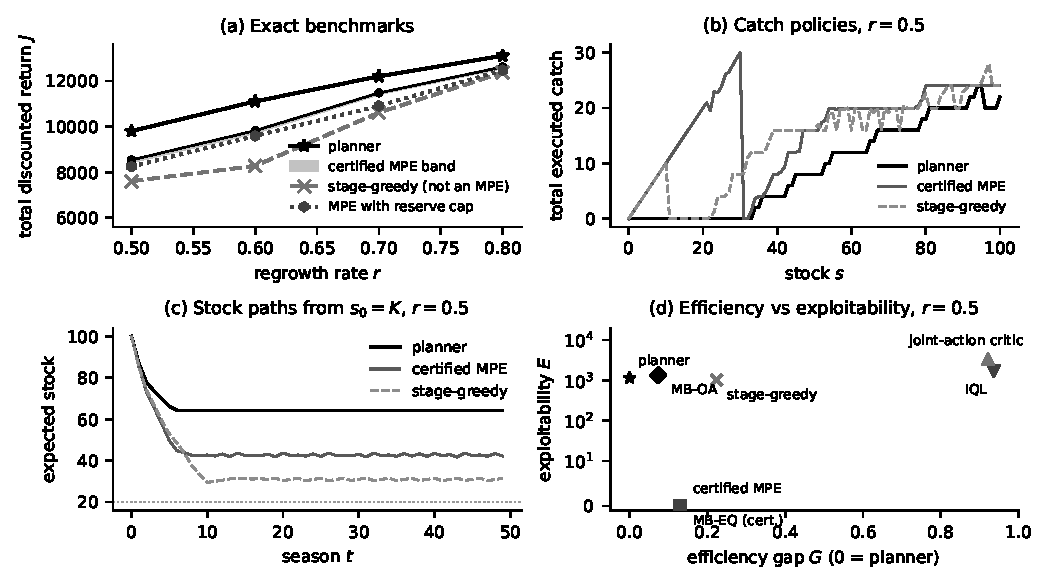
\includegraphics[width=\linewidth]{fig_bench_frontier.pdf}
\caption{(a) Planner, certified MPE band, the stage-greedy profile and the capped (safe) MPE as functions of $r$.
(b) Stationary catch policies and (c) expected stock paths from $s_0=K$ at $r=0.5$ (dotted: collapse threshold $\delta K$).
(d) Every profile and learner at $r=0.5$ by efficiency gap and exploitability (symmetric log scale): the planner is
efficient but exploitable, equilibria are unexploitable but inefficient, MB-OA sits near the planner.}
\label{fig:bench}
\end{figure}

\subsection{Learners in self-play (Q1, Q2)}
Table~\ref{tab:learners} and Figure~\ref{fig:curves} summarise self-play after training. Independent Q-learning ends far
below every equilibrium ($G=0.90$--$0.94$) and the stock collapses in 96--100\% of evaluation runs. Its learning cost
per episode, $\bar L_\tau$ against the planner, is 3.4--4.1 times that of MB-OA. A shared team reward does not help
(Team-IQL $G\approx0.95$), so the failure comes from decentralised exploration, not from selfish incentives. The tabular
joint-action critic is only slightly better ($G=0.78$ at $r=0.8$). MB-EQ reaches exactly the equilibrium it is told to
play: with a certified MPE it gets the MPE value with collapse at most 2\% and $E\le2$; with the stage-greedy profile it
inherits that profile's exploitability and its collapse rate of 38\% at $r=0.6$. MB-OA settles closest to the planner
($G=0.023$--$0.074$, no collapse) in 200 episodes, but in self-play it is exploitable ($E=708$--$1339$): each fleet best
responds to a model of a cooperative-looking opponent, so neither is at an equilibrium.
Patience and noise matter as Q1 anticipated (collapse rates averaged over $r$): with $\gamma=0.90$ MB-EQ collapses the
stock in 90--100\% of runs and with $\sigma=0.2$ in 61\% even at $\gamma=0.99$, whereas MB-OA keeps collapse at or below
0.1\% whenever $\sigma\le0.1$ and at 7\% for $\sigma=0.2$, $\gamma=0.99$.

\begin{table}[h]
\centering
\caption{Self-play after training: $G$ / $C_{50}$ / $E$ (means over 20 seeds; $\gamma=0.99$, $\sigma=0.1$).}
\label{tab:learners}
\small
\begin{tabular}{lcccc}
\toprule
Learner (episodes) & $r=0.5$ & $r=0.6$ & $r=0.7$ & $r=0.8$ \\
\midrule
IQL (5000) & 0.937 / 1.00 / 1{,}714 & 0.936 / 1.00 / 3{,}078 & 0.922 / 0.99 / 4{,}559 & 0.903 / 0.96 / 5{,}774 \\
MB-EQ, certified MPE (500) & 0.130 / 0.02 / 0 & 0.119 / 0.02 / 0 & 0.060 / 0.00 / 1 & 0.041 / 0.00 / 2 \\
MB-EQ, stage-greedy profile (500) & 0.224 / 0.01 / 1{,}030 & 0.255 / 0.38 / 272 & 0.131 / 0.00 / 95 & 0.056 / 0.00 / 11 \\
MB-OA (200) & 0.074 / 0.00 / 1{,}339 & 0.055 / 0.00 / 1{,}246 & 0.045 / 0.00 / 1{,}110 & 0.023 / 0.00 / 708 \\
Joint-action critic (5000) & 0.922 / 0.99 / 3{,}339 & 0.901 / 0.93 / 4{,}944 & 0.870 / 0.84 / 5{,}609 & 0.776 / 0.54 / 5{,}652 \\
Team-IQL (5000) & 0.955 / 1.00 / 1{,}123 & 0.957 / 1.00 / 1{,}799 & 0.958 / 1.00 / 3{,}319 & 0.951 / 1.00 / 4{,}707 \\
\bottomrule
\end{tabular}

\end{table}

\begin{figure}[h]
\centering
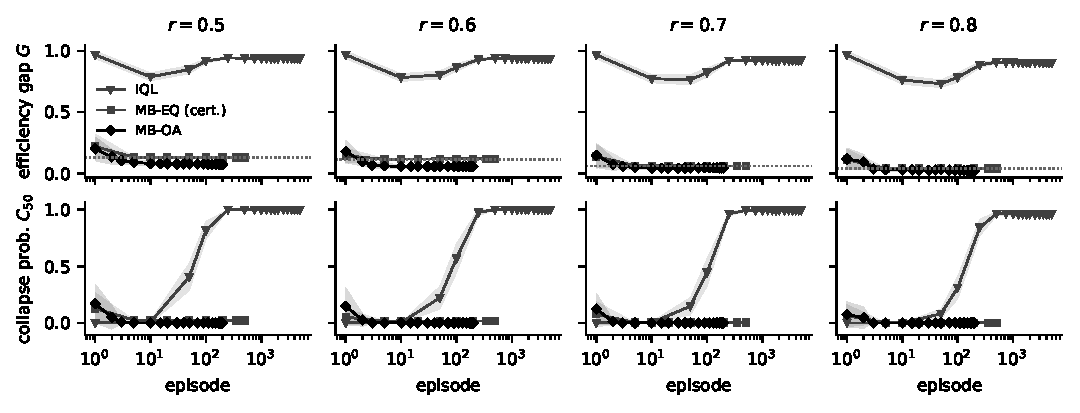
\includegraphics[width=\linewidth]{fig_curves.pdf}
\caption{Learning curves: efficiency gap (top; dotted: best certified MPE) and evaluation collapse probability (bottom),
mean and 95\% interval over 20 seeds.}
\label{fig:curves}
\end{figure}

\subsection{Responding to the other fleet (review feedback 1)}
Table~\ref{tab:cross} pairs MB-OA and MB-EQ against the same opponent, seed and noise. Against an over-harvester MB-OA
lowers its own request and gains $+1436.5\pm331.3$ (pooled), up to $+3702.1$ at $r=0.8$ where MB-EQ collapses the stock.
Against an equilibrium player it loses a little own return (significantly, $-31$ to $-672$, except a gain of $+106$ at
$r=0.6$) while raising joint efficiency ($\Delta G=-0.12$ pooled): it best-responds rather than defends.
Against another MB-OA it earns 1038 less than MB-EQ would (pooled), consistent with its exploitability in
Table~\ref{tab:learners}. Opponent
modelling therefore pays exactly when the opponent departs from the equilibrium.

\begin{table}[h]
\centering
\caption{Paired difference in own return, MB-OA minus MB-EQ, by opponent and $r$ ($^{*}$: Holm-adjusted $p<0.05$, 24 tests).
$^{\dagger}$The IQL opponent trains for 200 episodes when paired with MB-OA but 500 when paired with MB-EQ, so this row is
not a like-for-like comparison.}
\label{tab:cross}
\small
\begin{tabular}{lccccc}
\toprule
Opponent & $r=0.5$ & $r=0.6$ & $r=0.7$ & $r=0.8$ & pooled (95\% CI) \\
\midrule
MB-EQ & -671.5$^{*}$ & +106.5$^{*}$ & -31.0$^{*}$ & -97.9$^{*}$ & -173.5 $\pm$ 69.5 \\
MB-OA & -1{,}540.2$^{*}$ & -1{,}253.6$^{*}$ & -838.6$^{*}$ & -521.3$^{*}$ & -1{,}038.4 $\pm$ 167.5 \\
IQL$^{\dagger}$ & +2.0 & +19.3 & +20.4 & -299.7 & -64.5 $\pm$ 101.9 \\
Planner share & -34.3$^{*}$ & +45.2$^{*}$ & +100.2$^{*}$ & +99.4$^{*}$ & +52.6 $\pm$ 12.3 \\
Stage-greedy profile & -718.8$^{*}$ & +138.3$^{*}$ & -8.1$^{*}$ & -70.7$^{*}$ & -164.8 $\pm$ 74.3 \\
Over-harvester ($a=14$) & +52.5$^{*}$ & +185.2$^{*}$ & +1{,}806.2$^{*}$ & +3{,}702.1$^{*}$ & +1{,}436.5 $\pm$ 331.3 \\
\bottomrule
\end{tabular}

\end{table}

\subsection{Not knowing $r$, and the amount of data (Q3)}\label{sec:unknownr}
The posterior puts all its mass within $0.05$ of the true $r$ in every run. Paired by seed, the first-episode cost of not
knowing $r$ is small ($-44.7\pm33.8$ at $r=0.5$, about 2\% of an episode's return) and not distinguishable from zero at
$r=0.6$ and $0.8$; after that the belief-based and known-$r$ learners are indistinguishable ($G=0.224$ both at $r=0.5$).
The 11.6--18.1\% of runs that collapse during the exploratory warm-up do so equally with and without knowledge of $r$.
The data sweep agrees that the warm-up length is what matters: without warm-up MB-OA training collapse is 0--0.7\%,
against 13.0\% with 5 warm-up seasons and 84.0\% with 50, while the re-planning interval and the prior width change the
final $G$ by at most 0.014.

\textbf{When the true $r$ was never solved.} MB-EQ plays the equilibrium interpolated between the values of $r$ that were
solved in advance, and in all experiments above the true $r$ is one of them. Evaluating exactly the policy MB-EQ converges
to when the true $r$ lies between solved values (E12), at $r=0.55$, $0.65$ and $0.75$ it loses 1.9\%, 1.7\% and 0.7\% of
welfare against the certified MPE at that $r$, and a fleet gains 1.5\%, 0.7\% and 0.3\% of its value by deviating.
Interpolating equilibria is therefore a mild but real approximation; solving at the posterior mean removes it.

\subsection{Safety: what the reserve cap costs (Q3)}
Table~\ref{tab:safety} separates who pays for the reserve cap. The cap never binds for the planner (zero cost). For
selfish fleets it removes the equilibrium's residual collapse risk (up to 3.6\%) but lowers the equilibrium value by
142--563. The capped equilibrium is itself certified (an exact equilibrium at $r=0.5$, an $\varepsilon$-equilibrium with
$\varepsilon\le0.2\%$ of value at $r\ge0.6$). The cap is a safety instrument, not an efficiency one: it does not move
selfish fleets towards the planner. Learners trained under the cap have no collapse in training or evaluation.

\begin{table}[H]
\centering
\caption{Reserve cap ($S_{\text{res}}=25$): planner and best certified MPE without and with the cap, and the MPE collapse rate.}
\label{tab:safety}
\small
\begin{tabular}{cccccccc}
\toprule
 & \multicolumn{2}{c}{Planner} & \multicolumn{2}{c}{Best certified MPE} & Cost of cap & \multicolumn{2}{c}{$C_{50}$ of MPE} \\
$r$ & uncapped & capped & uncapped & capped & (equilibrium) & uncapped & capped \\
\midrule
0.5 & 9{,}802.5 & 9{,}802.5 & 8{,}532.6 & 8{,}246.1 & +286.6 & 0.036 & 0.000 \\
0.6 & 11{,}103.6 & 11{,}103.6 & 9{,}821.2 & 9{,}589.3 & +232.0 & 0.008 & 0.000 \\
0.7 & 12{,}204.1 & 12{,}204.1 & 11{,}474.4 & 10{,}911.5 & +562.9 & 0.004 & 0.000 \\
0.8 & 13{,}106.6 & 13{,}106.6 & 12{,}614.7 & 12{,}472.3 & +142.3 & 0.000 & 0.000 \\
\bottomrule
\end{tabular}

\end{table}

\subsection{Can cooperation be sustained? (Q4)}\label{sec:coop}
\IfFileExists{tables/tab_coop.tex}{%
Table~\ref{tab:coop} and Figure~\ref{fig:coop} give the exact grim-trigger threshold. Cooperation at the planner's
catch \emph{can} be sustained as a subgame-perfect equilibrium: Eq.~\eqref{eq:grim} holds at every stock if and only if
$\gamma\ge\gamma^*(r)$, with $\gamma^*$ between 0.77 ($r=0.5$) and 0.68 ($r=0.8$), far below the $\gamma=0.99$ we study.
The binding stocks are low ones ($s\approx7$--$12$), where the planner lets the stock rebuild and a deviator could take
what is left; a one-season deviation gains little elsewhere because the cost is convex, while punishment loses the value
of cooperation for good. $\gamma^*$ falls as $r$ rises because faster regrowth shortens the rebuilding the cooperative
path asks for. At every $\gamma$ near the threshold the punishment equilibrium passes the certificate ($E\le0.07$).

The learners do not find this cooperation. Under a forced one-season over-harvest, memory-one learners cut their next
catch by 3.3--3.7, but at the same stock their catch after a deviation differs by about one unit or less, and the regime
bit fires by construction (the probe catch is above the trigger threshold). The cut follows the lower stock, not a
learned punishment. Sustaining cooperation therefore requires the strategy to be designed or computed, not discovered by
tabular Q-learning in 5000 episodes.
\begin{figure}[h]
\centering
\begin{minipage}[c]{0.40\linewidth}
\centering
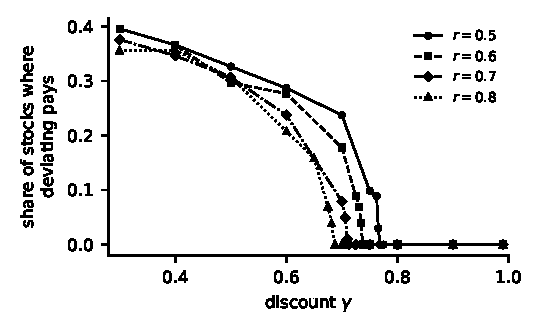
\includegraphics[width=\linewidth]{fig_coop.pdf}
\captionof{figure}{Share of stocks at which a one-season deviation from cooperation pays, against $\gamma$. Zero means
the grim trigger is a subgame-perfect equilibrium.}
\label{fig:coop}
\end{minipage}\hfill
\begin{minipage}[c]{0.57\linewidth}
\centering
\captionof{table}{Exact grim-trigger threshold (cooperation = symmetric planner, punishment = certified MPE) and the
memory-one probe (same-stock catch after a deviation minus without; negative = restraint).}
\label{tab:coop}
\scriptsize
\begin{tabular}{cccc}
\toprule
$r$ & $\gamma^*$ (SPE iff $\gamma\ge\gamma^*$) & $J^{\text{coop}}-J^{*}$ ($\gamma=0.99$) & memory-one gap \\
\midrule
0.5 & 0.767 $\pm$ 0.002 & +1{,}266.6 & -1.29 $\pm$ 1.12 \\
0.6 & 0.736 $\pm$ 0.002 & +1{,}279.3 & -1.00 $\pm$ 0.94 \\
0.7 & 0.711 $\pm$ 0.002 & +725.2 & -0.12 $\pm$ 0.78 \\
0.8 & 0.684 $\pm$ 0.003 & +518.8 & -0.24 $\pm$ 1.20 \\
\bottomrule
\end{tabular}

\end{minipage}
\end{figure}}{}

\subsection{Answers and limitations}
\textbf{Q1:} independent learners settle far below any equilibrium; model-based learners reach the equilibrium they
play; opponent-aware learners settle near the planner but are exploitable. \textbf{Q2:} a model plus exact planning
matters more than a centralised critic: MB-OA has a 3.4--4.1$\times$ lower learning cost than IQL, and the joint-action
critic barely improves on IQL. \textbf{Q3:} not knowing $r$ costs little once the belief is used. The warm-up exploration,
not the uncertainty, causes collapse during learning, and a reserve cap removes collapse at a welfare cost borne only by
selfish play. \textbf{Q4:} cooperation is sustainable as a subgame-perfect equilibrium for $\gamma\ge\gamma^*\approx0.68$--$0.77$,
but memory-one learners do not learn it.
\textbf{Limitations.} Two fleets only (three fleets and the neural actor-critic, planned as optional extensions, were not run); a stylised growth law;
grid discretisation (a finer catch grid moves the certified equilibrium value by under 2\%); symmetric mixed equilibria
are enumerated only with support size 2; independent learners have no convergence guarantee (their non-convergence is
reported as a result); the learning experiments use true $r$ values that were solved in advance (Section~\ref{sec:unknownr}
measures the cost otherwise); the IQL opponent's training budget differs between the two compared learners in
Table~\ref{tab:cross}.


%------------------------------------------------------------
\section{Contribution}
\label{sec:contrib}
%------------------------------------------------------------
Table~\ref{tab:work} lists each member's tasks from the project review, whether they were fulfilled, and what each member delivered. All members took part in writing and reviewing the report. The repository, with a README, run instructions and screenshots of the results, is at \url{https://github.com/ParamTanna/Fishery-Marl}; every table and figure in Section~\ref{sec:results} is regenerated from the raw results by the scripts in it.

\begin{table}[H]
  \centering
  \caption{Division of work and fulfilment.}
  \label{tab:work}
  \small
  \begin{tabular}{p{3.0cm}p{5.0cm}p{1.2cm}p{5.5cm}}
    \toprule
    Member & Tasks (project review) & Fulfilled & Delivered \\
    \midrule
    Panchal Heet Chirag & Environment and planner: fishery dynamics, rationing rule, discretisation, planner dynamic program, closed-form check & Yes & environment and quadrature, planner, Levhari--Mirman check (0.95\%), regime sweep and benchmark runs (E0, E1) \\
    Param Tanna & Equilibrium solvers: backward induction, stage-game solver, distance-to-equilibrium measure, cooperation and punishment analysis & Yes & equilibrium solver with seven selection rules, exact best responses and certificate, Price of Anarchy and Stability, safety and cooperation analysis (E8, E10--E12), integration of the results pipeline, repository and report \\
    Mehul Prakash Parakh & Tabular and model-based learners: independent Q-learning, estimation of $r$ and beliefs & Yes & IQL, Bayesian belief, MB-EQ, the opponent-aware MB-OA (review feedback 1), tuning, and learning experiments (E2--E4, E6, E7) \\
    Pawar Sai Tejeshwar & Neural learners and experiments: actor-critic, centralised critic, team-reward baseline, experiment runs and plots & Partly & team baselines (E5) and tabular joint-action critic (E9); the neural actor-critic was not done \\
    \bottomrule
  \end{tabular}
\end{table}

%Bibliography
{\small
\begin{thebibliography}{99}
\setlength{\itemsep}{0.5pt}

\bibitem{hardin1968}
G.~Hardin.
\newblock The tragedy of the commons.
\newblock \textit{Science}, 162(3859):1243--1248, 1968.

\bibitem{ostrom1990}
E.~Ostrom.
\newblock \textit{Governing the Commons: The Evolution of Institutions for Collective Action}.
\newblock Cambridge University Press, 1990.

\bibitem{shapley1953}
L.~S. Shapley.
\newblock Stochastic games.
\newblock \textit{Proceedings of the National Academy of Sciences}, 39(10):1095--1100, 1953.

\bibitem{levhari1980}
D.~Levhari and L.~J. Mirman.
\newblock The great fish war: an example using a dynamic Cournot-Nash solution.
\newblock \textit{The Bell Journal of Economics}, 11(1):322--334, 1980.

\bibitem{littman1994}
M.~L. Littman.
\newblock Markov games as a framework for multi-agent reinforcement learning.
\newblock In \textit{Proceedings of ICML}, 1994.

\bibitem{tan1993}
M.~Tan.
\newblock Multi-agent reinforcement learning: independent vs. cooperative agents.
\newblock In \textit{Proceedings of ICML}, 1993.

\bibitem{watkins1992}
C.~J. C.~H. Watkins and P.~Dayan.
\newblock Q-learning.
\newblock \textit{Machine Learning}, 8(3-4):279--292, 1992.

\bibitem{hu2003}
J.~Hu and M.~P. Wellman.
\newblock Nash Q-learning for general-sum stochastic games.
\newblock \textit{Journal of Machine Learning Research}, 4:1039--1069, 2003.

\bibitem{zhang2021}
K.~Zhang, Z.~Yang, and T.~Ba\c{s}ar.
\newblock Multi-agent reinforcement learning: a selective overview of theories and algorithms.
\newblock In \textit{Handbook of Reinforcement Learning and Control}, Springer, 2021.

\bibitem{lowe2017}
R.~Lowe, Y.~Wu, A.~Tamar, J.~Harb, P.~Abbeel, and I.~Mordatch.
\newblock Multi-agent actor-critic for mixed cooperative-competitive environments.
\newblock In \textit{Advances in Neural Information Processing Systems (NeurIPS)}, 2017.

\bibitem{sutton2018}
R.~S. Sutton and A.~G. Barto.
\newblock \textit{Reinforcement Learning: An Introduction}.
\newblock MIT Press, 2nd edition, 2018.

\bibitem{leibo2017}
J.~Z. Leibo, V.~Zambaldi, M.~Lanctot, J.~Marecki, and T.~Graepel.
\newblock Multi-agent reinforcement learning in sequential social dilemmas.
\newblock In \textit{Proceedings of AAMAS}, 2017.

\bibitem{perolat2017}
J.~Perolat, J.~Z. Leibo, V.~Zambaldi, C.~Beattie, K.~Tuyls, and T.~Graepel.
\newblock A multi-agent reinforcement learning model of common-pool resource appropriation.
\newblock In \textit{Advances in Neural Information Processing Systems (NeurIPS)}, 2017.

\bibitem{maskin2001}
E.~Maskin and J.~Tirole.
\newblock Markov perfect equilibrium: I. Observable actions.
\newblock \textit{Journal of Economic Theory}, 100(2):191--219, 2001.

\bibitem{dutta1993}
P.~K. Dutta and R.~K. Sundaram.
\newblock The tragedy of the commons?
\newblock \textit{Economic Theory}, 3(3):413--426, 1993.

\bibitem{howard1960}
R.~A. Howard.
\newblock \textit{Dynamic Programming and Markov Processes}.
\newblock MIT Press, 1960.

\bibitem{lemke1964}
C.~E. Lemke and J.~T. Howson.
\newblock Equilibrium points of bimatrix games.
\newblock \textit{Journal of the Society for Industrial and Applied Mathematics}, 12(2):413--423, 1964.

\bibitem{harsanyi1988}
J.~C. Harsanyi and R.~Selten.
\newblock \textit{A General Theory of Equilibrium Selection in Games}.
\newblock MIT Press, 1988.

\bibitem{koutsoupias1999}
E.~Koutsoupias and C.~Papadimitriou.
\newblock Worst-case equilibria.
\newblock In \textit{Proceedings of STACS}, pages 404--413, 1999.

\bibitem{anshelevich2004}
E.~Anshelevich, A.~Dasgupta, J.~Kleinberg, {\'E}.~Tardos, T.~Wexler, and T.~Roughgarden.
\newblock The price of stability for network design with fair cost allocation.
\newblock In \textit{Proceedings of FOCS}, pages 295--304, 2004.

\bibitem{fudenberg1986}
D.~Fudenberg and E.~Maskin.
\newblock The folk theorem in repeated games with discounting or with incomplete information.
\newblock \textit{Econometrica}, 54(3):533--554, 1986.

\bibitem{abreu1988}
D.~Abreu.
\newblock On the theory of infinitely repeated games with discounting.
\newblock \textit{Econometrica}, 56(2):383--396, 1988.

\bibitem{claus1998}
C.~Claus and C.~Boutilier.
\newblock The dynamics of reinforcement learning in cooperative multiagent systems.
\newblock In \textit{Proceedings of AAAI}, pages 746--752, 1998.

\bibitem{holm1979}
S.~Holm.
\newblock A simple sequentially rejective multiple test procedure.
\newblock \textit{Scandinavian Journal of Statistics}, 6(2):65--70, 1979.

\end{thebibliography}
}

\end{document}